\documentclass{sciposter}
\usepackage{epsfig}
\usepackage{amsmath}
\usepackage{amssymb}
\usepackage{multicol}
\usepackage{graphicx,url}
\usepackage{textpos}   
\usepackage[utf8]{inputenc}
\usepackage{xcolor}
\usepackage[ngerman]{babel}

\usepackage{tabularx}
\newcolumntype{L}[1]{>{\raggedright\arraybackslash}p{#1}} % linksbündig mit Breitenangabe
\newcolumntype{C}[1]{>{\centering\arraybackslash}p{#1}} % zentriert mit Breitenangabe
\newcolumntype{R}[1]{>{\raggedleft\arraybackslash}p{#1}} % rechtsbündig mit Breitenangabe

\usepackage{tikz}
\definecolor{rwth-blue}{HTML}{00549F}
\definecolor{rwth-lblue}{HTML}{8EBAE5}
\definecolor{rwth-llblue}{HTML}{C7DDF2}

% project title
\title{
	\leavevmode{
\includegraphics[scale=0.5]{../Logos/GestikulaserLogoBuntOhneSchrift.png}}\\
	Gestikulaser
}

% authors
\author{Christoph Behr, Cailing Fu, Nicole Grubert, Anna Pryadun, Daniel Wolff}

%\renewcommand\printleftlogo
%  {\begin{center}
%     \resizebox{\textwidth}{!}%
%       {
\includegraphics{TOSLogo.png}
\includegraphics{COSIMALogo.png}}
%   \end{center}
%  }
  
%\rightlogo[2]{TOSLogo.png}
%\leftlogo[2]{COSIMALogo}

% Section title color:
\definecolor{SectionCol}{rgb}{0.0, 0.329411, 0.62353} % RWTH Blau
% Section block color:
\definecolor{BoxCol}{rgb}{0.949,0.949,0.949} % Grau

\begin{document}

% TOS Logo oben links
\begin{textblock*}{60px}(0cm,0cm)
	
\includegraphics[height=4cm]{../Logos/TOS.eps}
\end{textblock*}

% COSIMA18 Logo oben rechts
\begin{textblock*}{60px}(55cm,0mm)
	
\includegraphics[height=4cm]{../Logos/Cosima18.png}
\end{textblock*}

\maketitle

%%% Begin of Multicols-Enviroment
\begin{multicols}{3}
\setlength{\parindent}{2em}

\section{Unsere Vision}
\noindent
Da die Interaktion zwischen Mensch und Computer immer mehr in unseren Alltag integriert wird, wird zunehmend versucht, diese Kommunikation möglichst natürlich zu gestalten. Hierbei spielen Gestenerkennungssysteme eine wichtige Rolle. \\
Mit dem Gestikulaser haben wir ein neues Gestenerkennungssystem entwickelt, um statische Handgesten eines Menschen zu erkennen und diese zur Interaktion mit einem Endgerät zu nutzen. Dabei soll der Gestikulaser nicht mit einer Kamera arbeiten, wie die meisten heute verfügbaren Systeme, sondern stattdessen soll die Hand des Nutzers mit Infrarot-LEDs beleuchtet und die Gesten durch die erzeugten Reflektionsmuster erkannt werden. Eine auf diese Weise realisierte Gestenerkennung ist nicht nur robust gegenüber sichtbaren Licht, sondern kann auch in vollkommener Dunkelheit betrieben werden. \\

% -----------------------------------------------------%

\section{Der Gestikulaser}
%Der Gestikulaser besteht aus zwei Komponenten, einer Photoplatte, sowie einer Machine Learning Software. \\
%Die Photoplatte ist mit mehreren infrarot LED Quellen, sowie einer Vielzahl von Photodioden ausgestattet, welche ausschließlich infrarotes Licht detektieren. Durch die Lichtreflexion der Hand oberhalb der Photoplatte können verschiedene Intensitäten an den Photodioden gemessen werden. Durch diese Intensitäten soll dann mit Hilfe der Machine Learning Software eine eindeutige Geste erkannt werden. Diese Geste kann dazu genutzt werden verschiedene Endgeräte, z.B. wie ein ferngesteuertes Auto oder eine Smart-Home Einrichtung zu steuern. \\
\noindent
\textbf{Hardware}
\begin{itemize}
	\item Photoplatte mit Photodioden und LEDs zur Beleuchtung der Hand und Detektion der reflektierten Strahlung
	\item Mikrocontroller zum Auslesen der Sensordaten
\end{itemize}

\noindent
\textbf{Software}
\begin{itemize}
	\item Verarbeiten der Sensordaten im Mikrocontroller und Kommunikation mit dem externen Computer
	\item Aufbau und Training eines neuronalen Netzmodells zur Erkennung der Gesten
\end{itemize}

\begin{figure}[h]
	\centering
	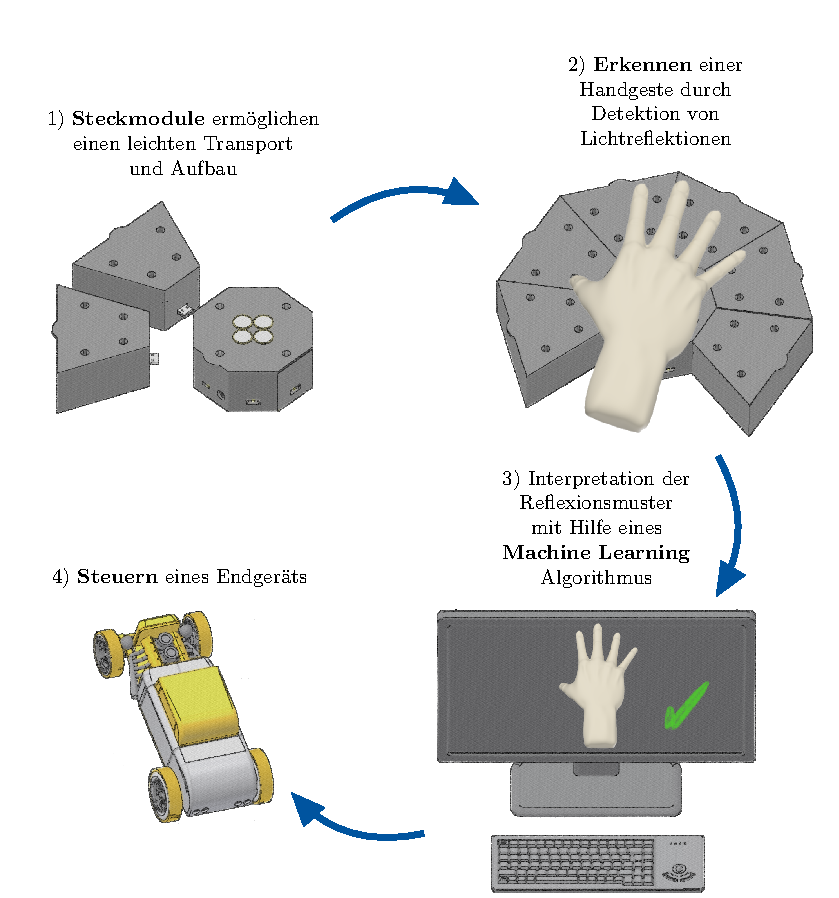
\includegraphics[scale=1.25]{../figures/tikz/GestikulaserAblauf.pdf}
	\caption{Schematischer Darstellung der Funktionsweise des Gestikulasers.}
	\label{fig:FunktionsweiseGestikulaser}
\end{figure}

% -----------------------------------------------------%

\section{Die Beta-Version}

\begin{itemize}
	\item Anordnung der Photodioden auf einer Pressspanplatte in einem festgelegten Muster
	\item Arduino Uno zur Auswertung der Sensordaten
	\item Maximal 16 Photodioden anschließbar
\end{itemize}

\begin{figure}[h]
	\centering
	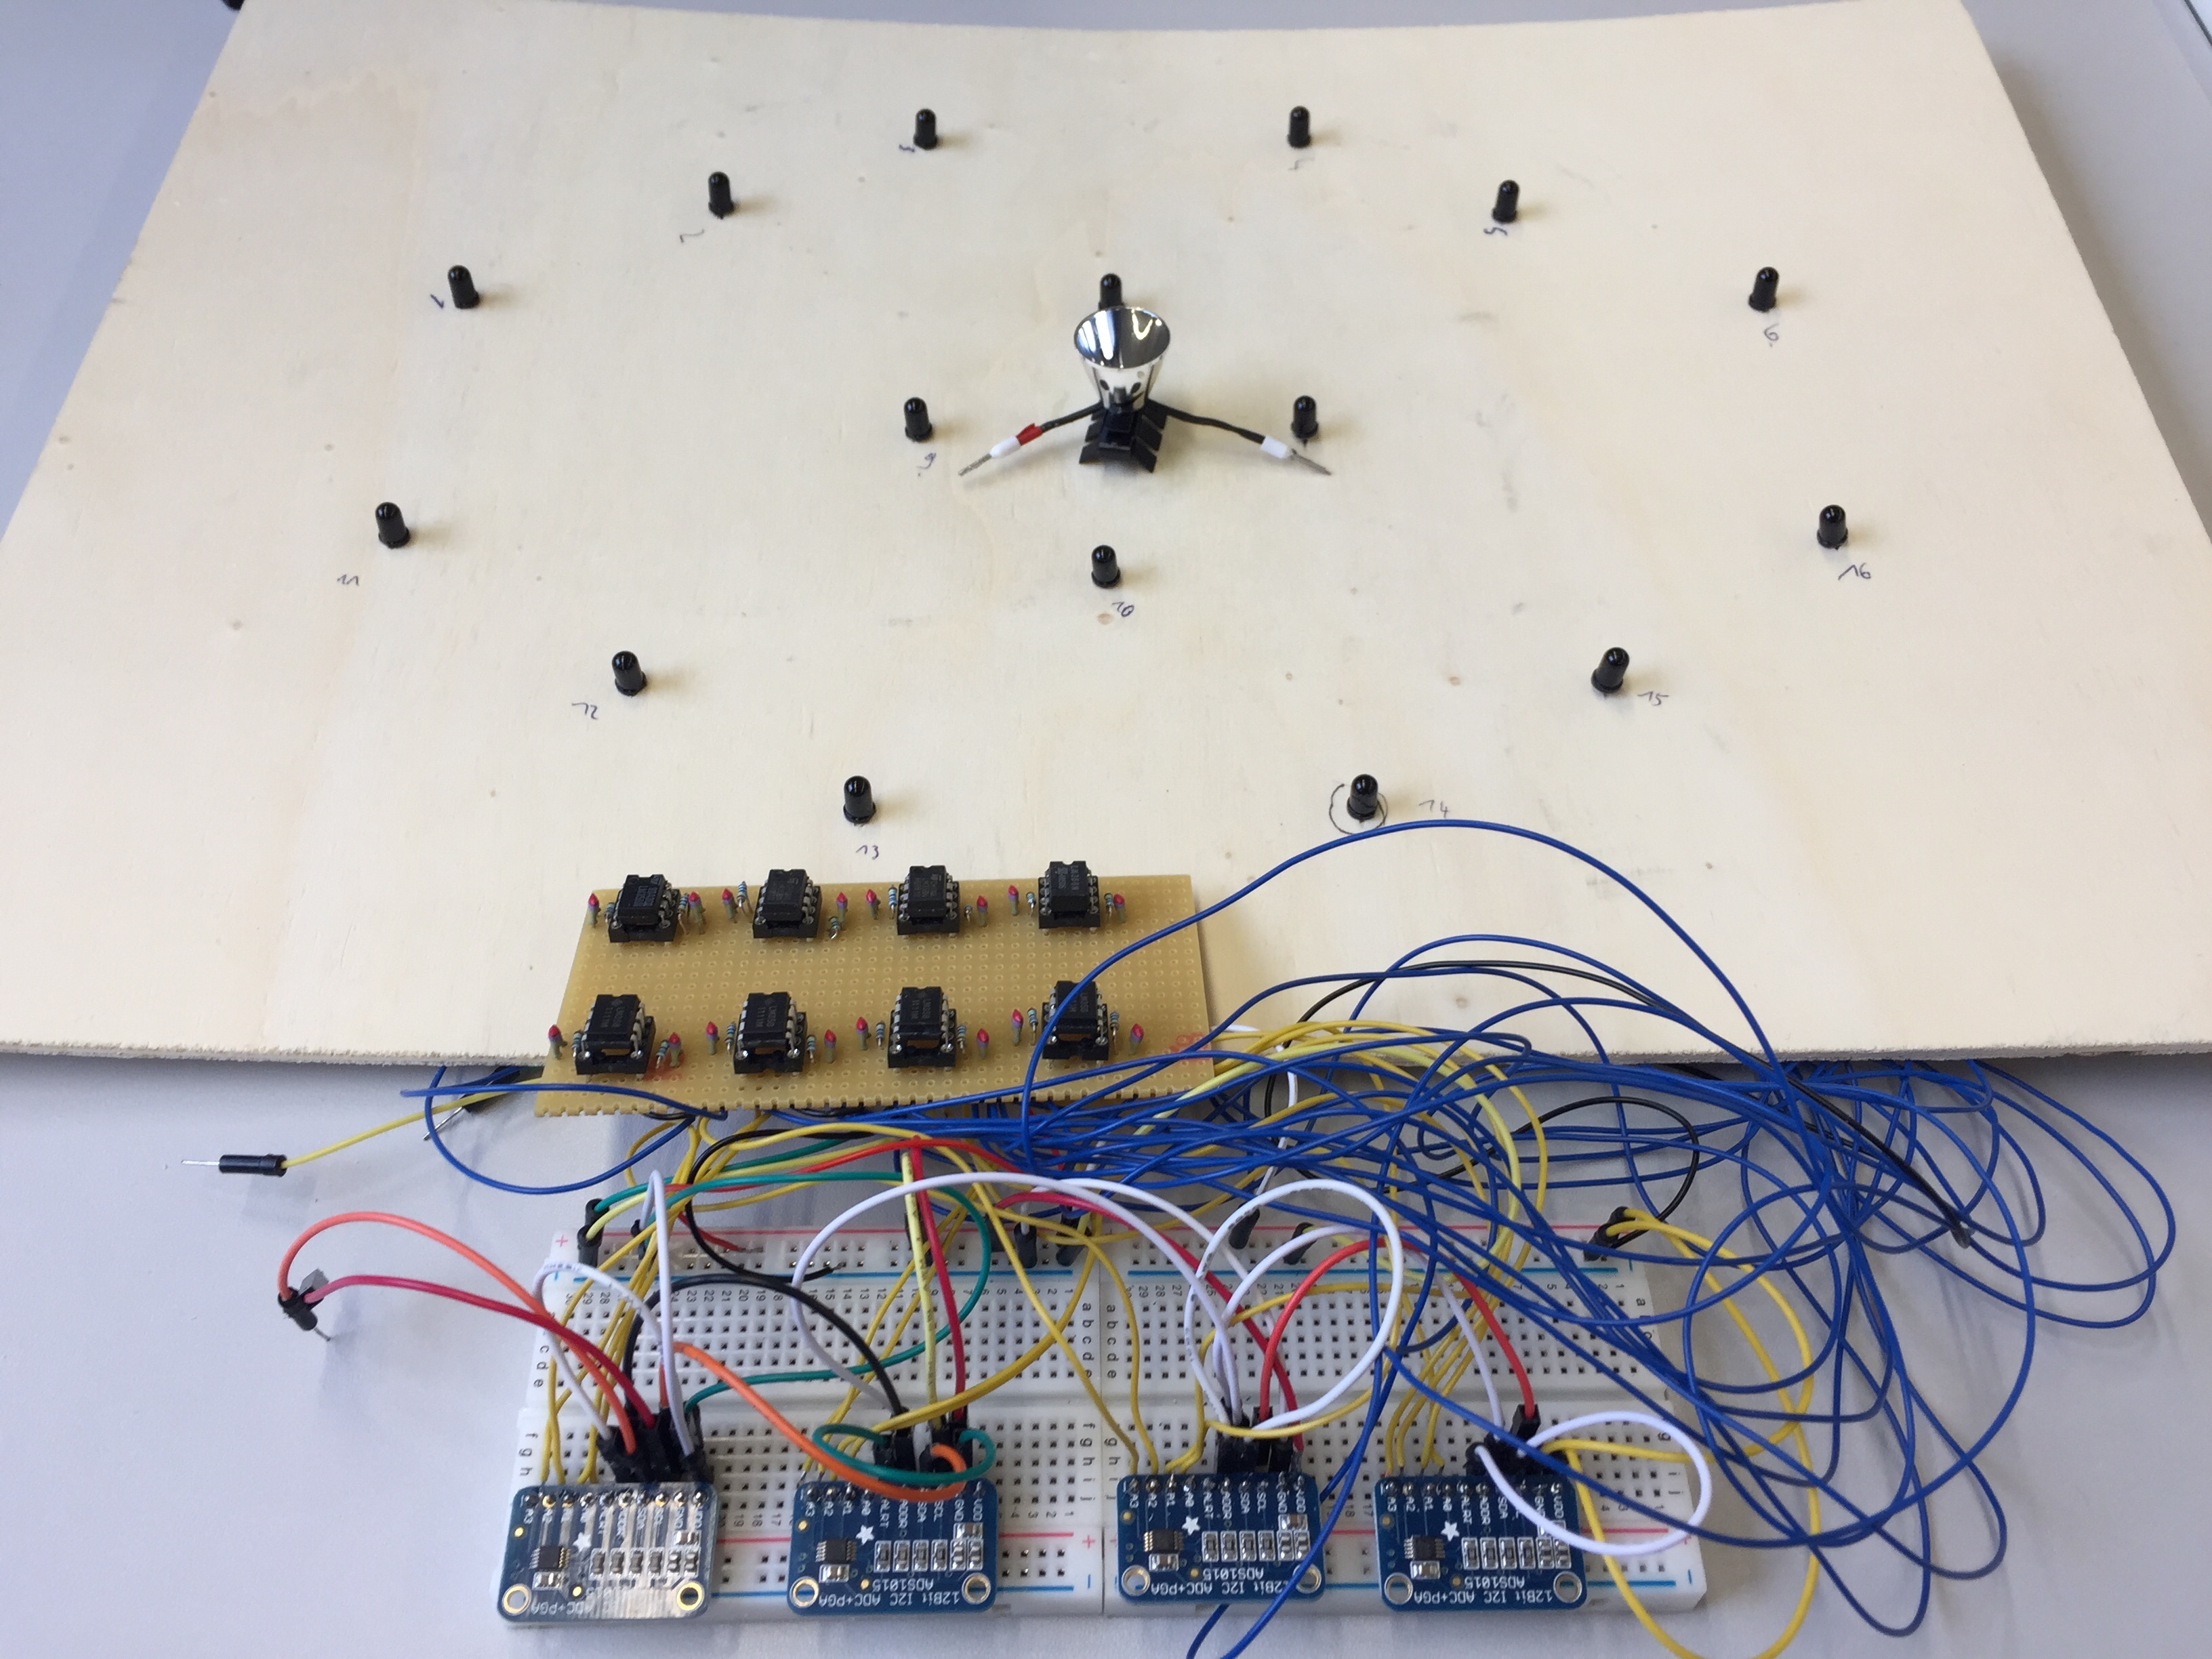
\includegraphics[scale=0.2]{../figures/PhotoplatteBeta.jpeg}
	\caption{Die Beta-Version der Photoplatte: Die Elektronik ist auf einer Steckplatine untergebracht, die Photodioden sind fest in der Platte verbaut.}
	\label{fig:PhotoplatteBeta}
\end{figure} \\
\noindent
Nachdem unsere Idee funktionierte, wollten wir nun unseren Gestikulaser modularer zu gestalten. Eine aus verschiedenen Steckmodulen zusammensetzbare Photoplatte sollte nun helfen, dieses Ziel zu erreichen.

% -----------------------------------------------------%

\section{Photoplatte}
\noindent
%Die neue Photoplatte besteht aus zwei verschiedenen Teilen, dem \textit{Oktokommander} als Herzstück der Photoplatte und passend dazu sieben \textit{Detektormodulen}. Die Detektormodule werden über USB-Anschlüsse an den Oktokommander angeschlossen. Der Microcontroller im Oktokommander wird mit einem zusätzlichen Datenkabel mit einem PC verbunden, auf dem die Software läuft.

\begin{itemize}
	\item Modulares Stecksystem aus insgesamt acht Komponenten
	\item Zentral gelegene, fest verbaute Lichtquelle
	\item Variable Anordnung der Photodioden
	\item Erweiterbar auf bis zu 128 Photodioden
\end{itemize}

\begin{figure}[h]
	\centering
	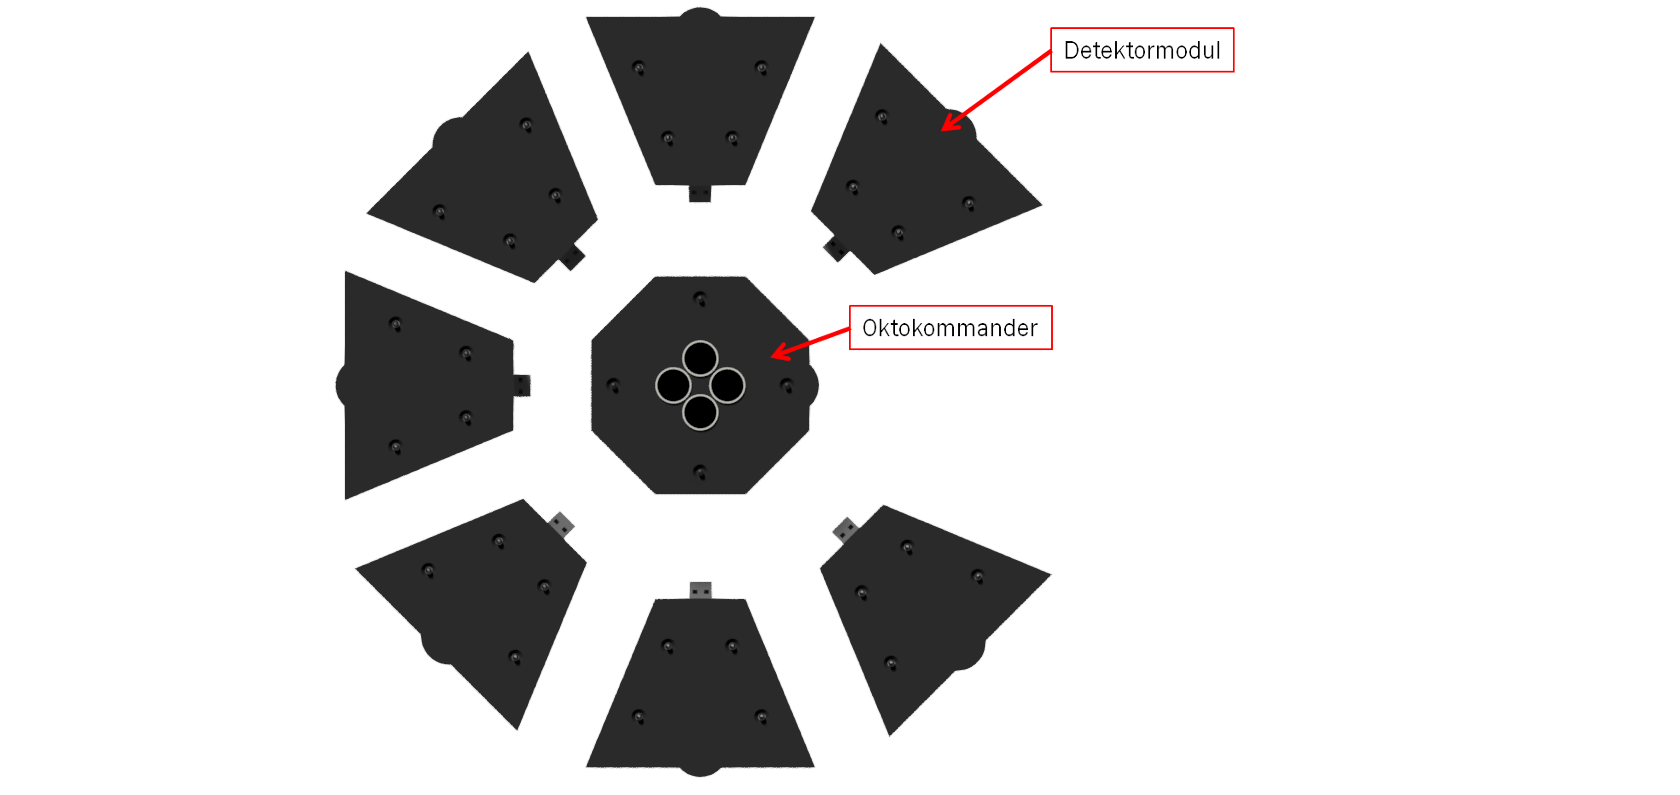
\includegraphics[scale=0.8]{../CAD_Bilder/Gestikulaser/Gestikulaser_raytraced_2_beschriftet.png}
	\caption{Die neue modulare Photoplatte setzt sich aus einem Oktokommander und bis zu sieben Detektormodulen zusammen.}
	\label{fig:PhotoplatteAlpha}
\end{figure}

% -----------------------------------------------------%

\section{Oktokommander}
\noindent
Der Oktokommander ist das Steuersystem der gesamten Photoplatte. Er enthält:
\begin{enumerate}
	\item Einen Arduino Micro
	\item Einen I2C Multiplexer
	\item Einen I2C AD-Wandler inklusive Verstärkerschaltung
	\item Vier Photodioden
	\item Vier infrarot LED Quellen
	\item Sieben USB-Anschlüsse für die Detektormodule
\end{enumerate}

\begin{figure}[h]
	\centering
	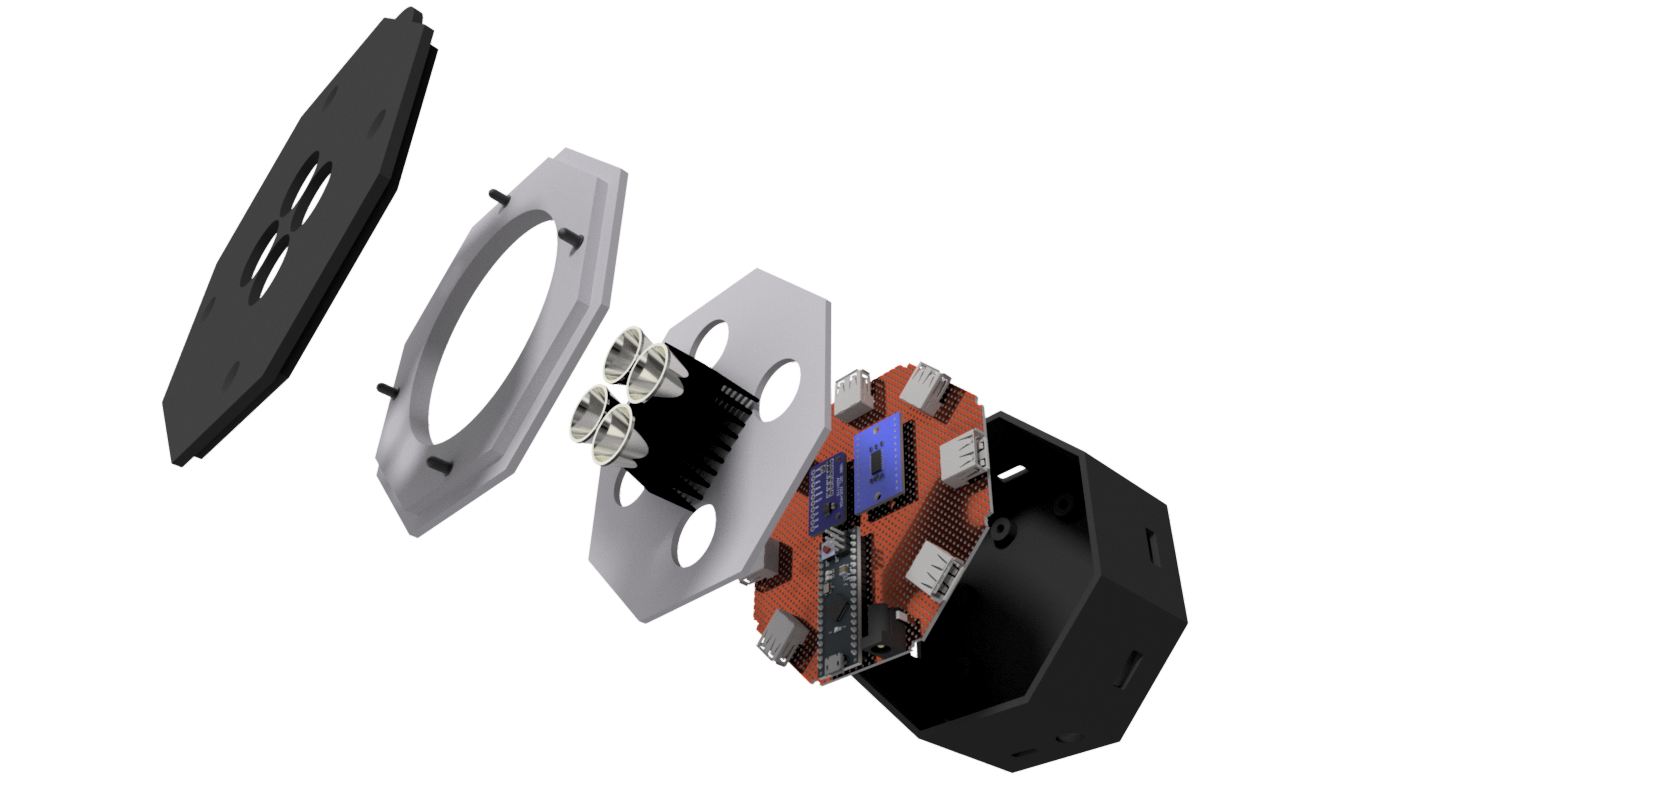
\includegraphics[scale=0.5]{../CAD_Bilder/Oktokommander/Oktokommander_raytraced.png}
	\caption{Explosionsdarstellung des Oktokommanders.}
	\label{fig:Oktokommander}
\end{figure}

% -----------------------------------------------------%

\section{Detektormodul}
\noindent
Die Detektormodule sollen die Lichtreflexionen der Hand detektieren. Sie enthalten jeweils:
\begin{enumerate}
	\item Vier Photodioden 
	\item Einen I2C AD-Wandler inklusive Verstärkerschaltung
	\item Einen USB-Stecker zum Anschluss an den Oktokommander
\end{enumerate}

\begin{figure}[h]
	\centering
	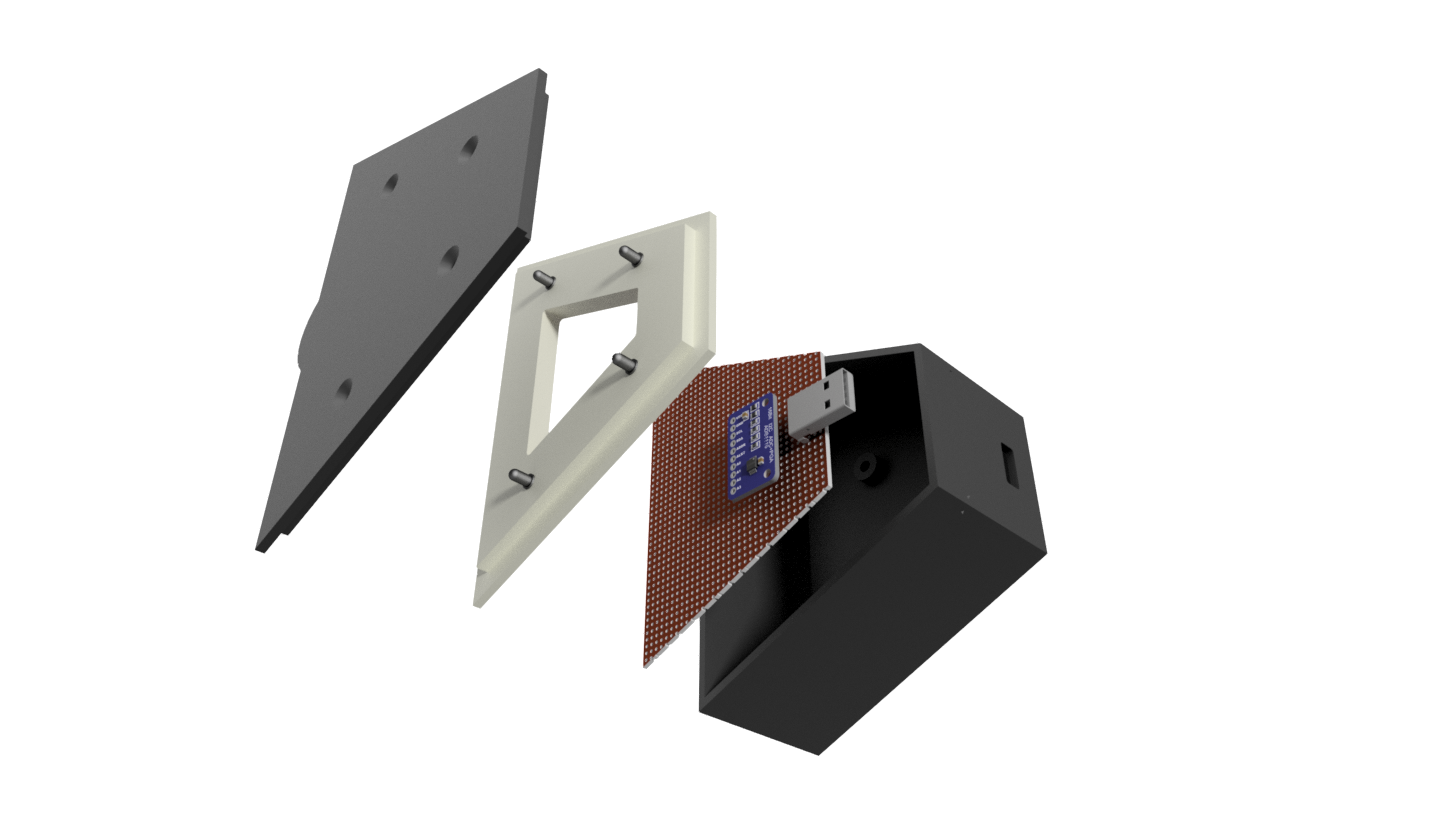
\includegraphics[scale=0.5]{../CAD_Bilder/Detektormodul/Detektormodul_raytraced.png}
	\caption{Explosionsdarstellung eines Detektormoduls.}
	\label{fig:Detektormodul}
\end{figure}

% -----------------------------------------------------%

\section{Software}
%Für den Gestikulaser wurden zwei Software Komponenten entwickelt: In der Trainingsphase nimmt der Nutzer Messdaten der Photodioden von zuvor definierten Gesten auf. Mit Hilfe dieser Daten wird dann ein neuronales Netz trainiert, das es im Live-Betrieb ermöglicht, direkt aus den gemessenen Sensordaten die vom Nutzer gemachte Geste zu bestimmen. Bei der verwendeten Software wurden nur open-source verfügbare Programme und Bibliotheken eingesetzt: Die Kommunikation zwischen dem Mikrocontroller und dem Computer erfolgt über \texttt{Python} Skripte, für die Erstellung des neuronalen Netzes wurde \texttt{TensorFlow}\texttrademark verwendet.

\noindent
Die Kommunikation zwischen dem Mikrocontroller und dem Computer erfolgt über \texttt{Python} Skripte, für die Erstellung des neuronalen Netzes wurde \texttt{TensorFlow}\texttrademark verwendet.

\noindent
%\begin{figure}
	\centering
\textbf{Trainingsphase}\\
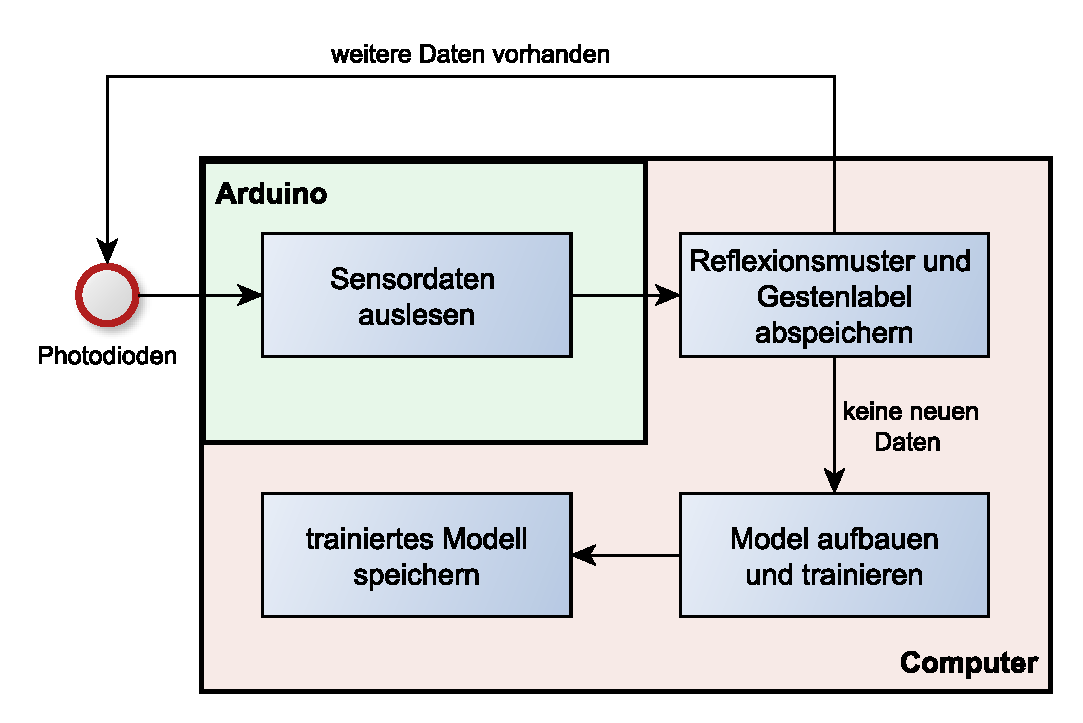
\includegraphics[scale=1]{../figures/AblaufTraining.pdf}
%\end{figure}
\noindent
\textbf{Live-Betrieb}\\
%\begin{figure}
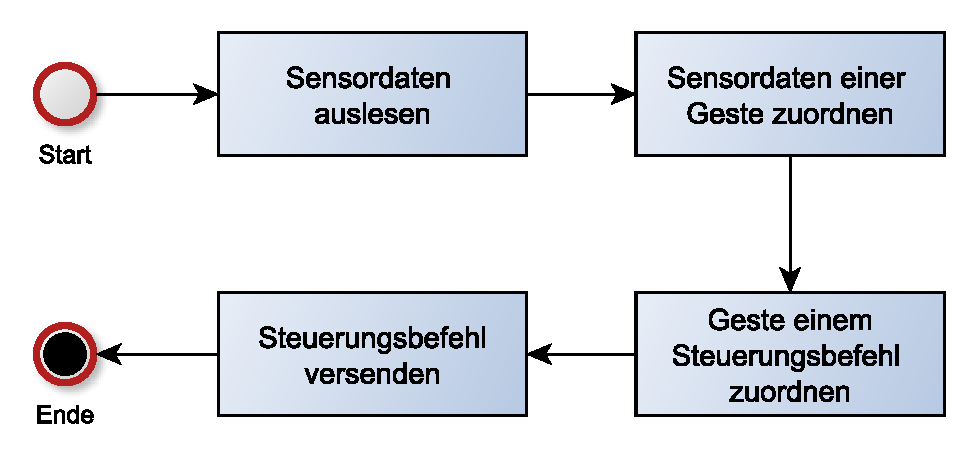
\includegraphics[scale=1]{../figures/AblaufSteuerung.pdf}
%\end{figure}

%\begin{tikzpicture}
%
%	%\clip (0,0) rectangle (18,-18);
%
%	\shadedraw[inner color=white, outer color=rwth-llblue] (0,0) rectangle (20,20);
%	\draw[help lines] (0,0) grid (20,20);
%	
%	\node[above] at (10,18.5) {\textbf{Trainingsphase}};
%	\node[below] at (10,19) {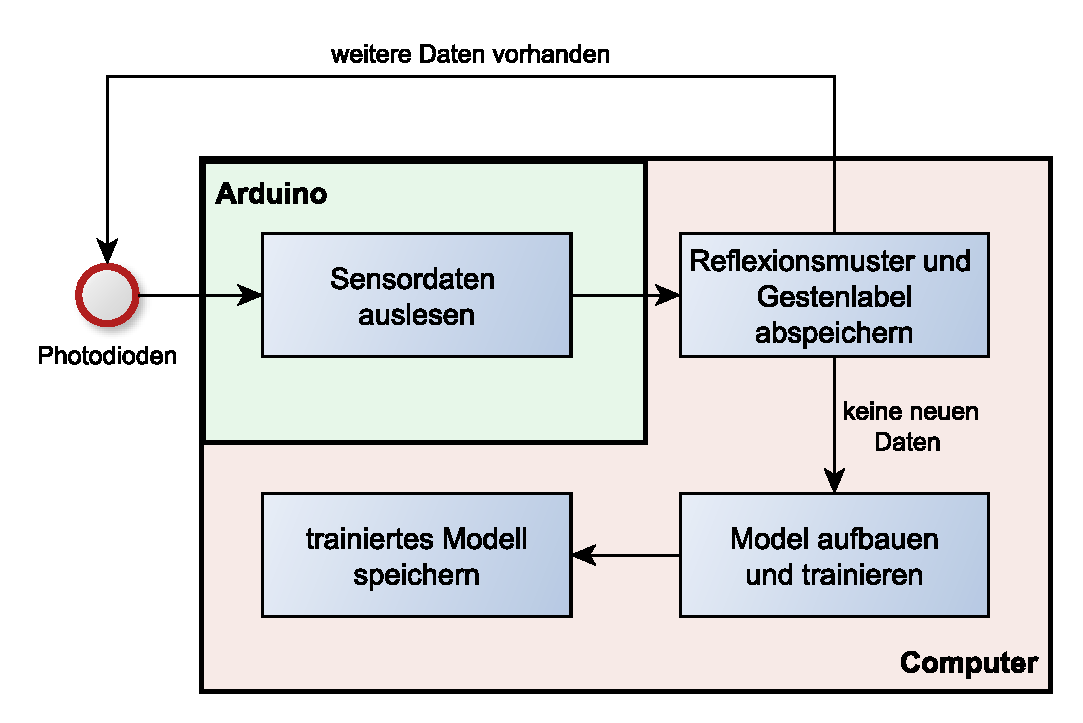
\includegraphics[scale=1]{../figures/AblaufTraining.pdf}};
%	
%	\node[above] at (10,5) {\textbf{Live-Betrieb}};
%	\node[below] at (10,5.5) {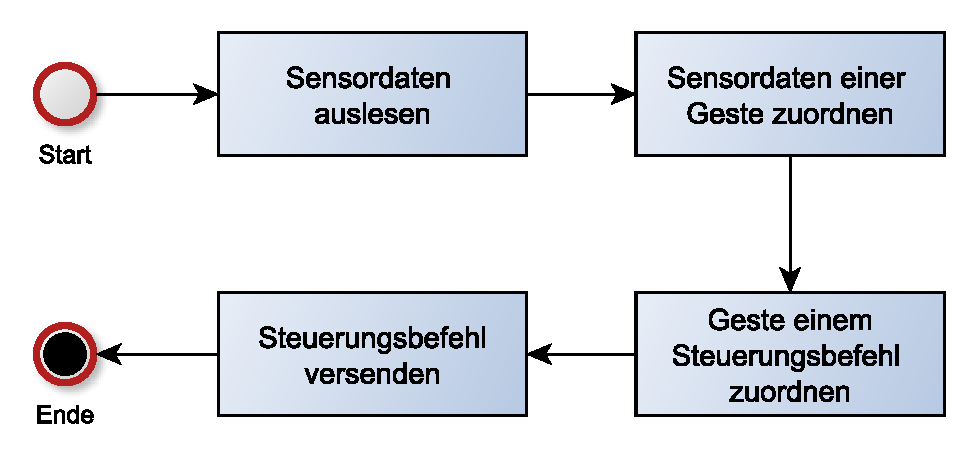
\includegraphics[scale=1]{../figures/AblaufSteuerung.pdf}};
%
%\end{tikzpicture}

%\begin{figure}[h]
%	\centering
%	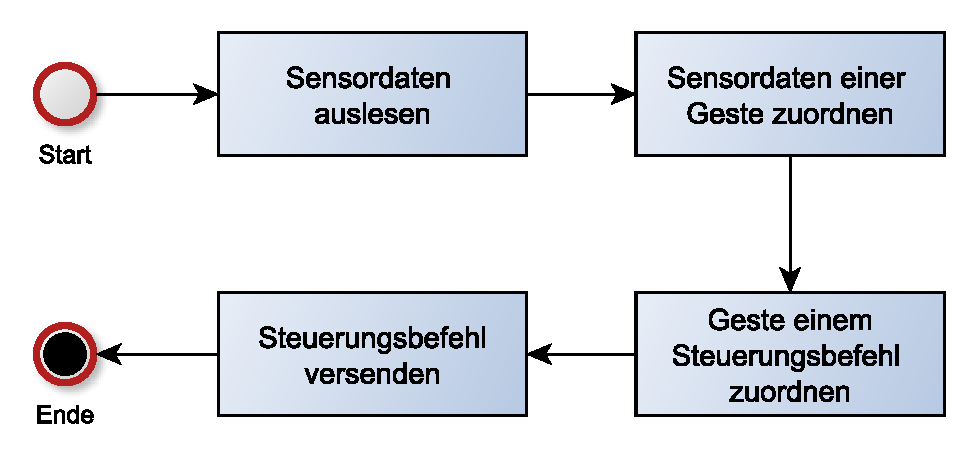
\includegraphics[scale=1]{../figures/AblaufSteuerung.pdf}
%	\caption{Ablaufdiagramm der Software im Live-Betrieb.}
%	\label{fig:AblaufSteuerung}
%\end{figure}

% -----------------------------------------------------%

\section{Ausblick}
\noindent
%Als Ausblick unseres Gestikulaser wäre eine Verfeinerung der aktuell durchführbaren Gestenerkennung denkbar, die nicht nur die Stellung der Hand, sondern auch die Krümmung der einzelnen Finger berücksichtigt. Zu diesem Zweck wurde bereits ein Prototyp für einen Sensorhandschuh entwickelt.

\begin{itemize}
	\item Erkennung feinerer Gesten durch Berücksichtigung der Krümmung der einzelnen Finger
	\item Erweiterung auf dynamische Gesten
	\item Erhöhung des Abstands durch mehr Lichtleistung
\end{itemize}

\begin{figure}[h]
	\centering
	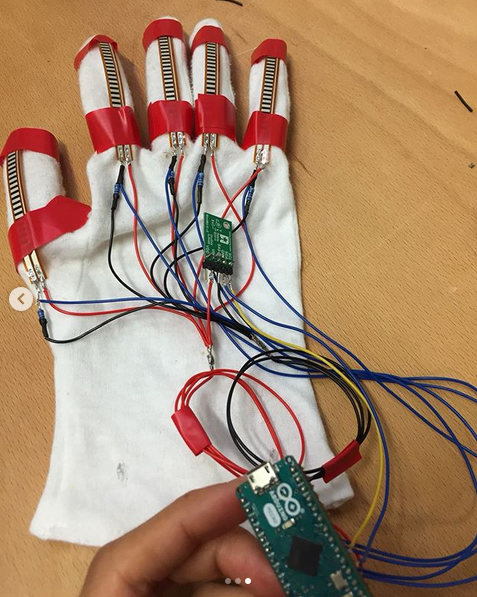
\includegraphics[scale=1.4]{../figures/Sensorhandschuh}
	\caption{Aktueller Prototyp eines Sensorhandschuhs. Es sind Biegesensoren für alle Finger, ein Gyroskop und ein Beschleunigungssensor im Einsatz. Die Sensordaten werden von einem Arduino Micro verarbeitet.}
	\label{fig:Sensorhandschuh}
\end{figure}

% -----------------------------------------------------%

\section{Sponsoren}
\noindent
Ein besonderen Dank gilt unseren Sponsoren: \\
\begin{tabularx}{\textwidth}{L{10cm} c}
	Aconity3D GmbH & \noindent\parbox[c]{\hsize}{
\includegraphics[height=3cm]{../Logos/AC3D_Logo_Print-for-white.eps}} \\
	& \\
	Fraunhofer ILT & \noindent\parbox[c]{\hsize}{
\includegraphics[height=3cm]{../Logos/Fraunhofer_ILT_klein.png}} \\
	& \\
	Würth Electronik \quad \quad GmbH Co. KG & \noindent\parbox[c]{\hsize}{
\includegraphics[height=3cm]{../Logos/Wuerth.png}}
\end{tabularx} \\

\end{multicols}

\conference{
	\raisebox{0.5cm}[0cm]{
\includegraphics[height=3cm]{../Logos/VDE.png} } \hfill
	\raisebox{1.25cm}[0cm]{
\includegraphics[height=1.5cm]{../Logos/Faulhaber.png}} \hfill
	\raisebox{0cm}[0cm]{
\includegraphics[height=4cm]{../Logos/micronit.png}} \hfill
	\raisebox{0cm}[0cm]{
\includegraphics[height=4cm]{../Logos/electronica.png}} \hfill 
	\raisebox{0cm}[0cm]{
\includegraphics[height=4cm]{../Logos/BMBF.png}}
}

\end{document}